\subsection{Observed Series and Validation Conditions}
The development-only diagnostics in Table~\ref{tab:data} agree with several visible patterns in Fig.~\ref{fig:series}. For carbon-dioxide levels, the ADF test did not reject a unit root, whereas KPSS rejected level stationarity. A first difference gave ADF $p<0.001$ and KPSS $p\geq0.10$. Retail levels showed the same opposing level-test outcomes. A twelve-month retail difference gave ADF $p=0.158$ and KPSS $p\geq0.10$; this did not establish stationarity. Rainfall gave ADF $p<0.001$ and KPSS $p\geq0.10$, consistent with an approximately stationary level over development. Sunspot levels gave ADF $p<0.001$ but KPSS $p=0.056$, while the plot revealed large amplitude changes between cycles. Power gave ADF $p=0.028$ and KPSS $p\geq0.10$; 23 missing daily targets still required the common causal-input rule. These results justified the declared transformations and cautioned against interpreting a single test as a complete description of a series. The five panels do not, by themselves, identify the mechanism of any later forecast error.

The split dates in Table~\ref{tab:splits} also matter for interpretation. The retail test began in August 2018 and included the sharp 2020--2021 movement visible in Fig.~\ref{fig:series}. The household test occupied only the last part of a roughly four-year record. Accordingly, the retail result tested a marked later disturbance, whereas the power result tested a comparatively short historical interval. Neither interval represents every plausible future operating condition.

\subsection{Selected Controls and Development Variation}
Table~\ref{tab:selection} reports the settings selected without consulting the final periods. The larger capacity budget was chosen in 13 of the 15 architecture-series combinations. The two small-budget choices were Elman for retail and Jordan for rainfall. No selected fold-seed fit had its best checkpoint at the 400-epoch cap.

\begin{table*}[t]
\caption{Selected controls from expanding development validation}
\label{tab:selection}
\centering\small
\begin{tabular}{llrrrrrr}
\toprule
Series & Network & Width & Parameters & Rate & Validation MAE & Refit epochs & Cap fits \\
\midrule
Carbon dioxide & Elman & 18 & 379 & 0.003 & 0.256 & 286 & 0 \\
Carbon dioxide & Jordan & 96 & 385 & 0.010 & 0.575 & 69 & 0 \\
Carbon dioxide & Combined & 18 & 397 & 0.010 & 0.270 & 64 & 0 \\
Sunspots & Elman & 18 & 379 & 0.010 & 18.993 & 14 & 0 \\
Sunspots & Jordan & 96 & 385 & 0.010 & 18.922 & 10 & 0 \\
Sunspots & Combined & 18 & 397 & 0.010 & 18.993 & 11 & 0 \\
Power & Elman & 18 & 379 & 0.010 & 0.212 & 17 & 0 \\
Power & Jordan & 96 & 385 & 0.010 & 0.219 & 28 & 0 \\
Power & Combined & 18 & 397 & 0.010 & 0.212 & 15 & 0 \\
Retail & Elman & 8 & 89 & 0.010 & 1.395 & 19 & 0 \\
Retail & Jordan & 96 & 385 & 0.010 & 1.383 & 12 & 0 \\
Retail & Combined & 18 & 397 & 0.003 & 1.427 & 14 & 0 \\
Rainfall & Elman & 18 & 379 & 0.010 & 29.427 & 12 & 0 \\
Rainfall & Jordan & 24 & 97 & 0.003 & 29.695 & 8 & 0 \\
Rainfall & Combined & 18 & 397 & 0.003 & 29.790 & 17 & 0 \\
\bottomrule
\end{tabular}
\end{table*}


The selected carbon-dioxide Elman network used 379 parameters, rate 0.003, and 286 refit epochs. Jordan used 385 parameters, rate 0.01, and 69 epochs; the combined network used 397 parameters, rate 0.01, and 64 epochs. Similar parameter counts did not produce similar validation MAE: Elman and combined feedback obtained 0.256 and 0.270 ppm, respectively, compared with Jordan's 0.575 ppm. The difference is consistent with a useful hidden-state feedback path for this transformed seasonal series, although capacity matching does not isolate feedback as a causal mechanism. Jordan's 96 hidden units also yielded a different optimisation geometry from Elman's 18.

Validation origins exposed temporal variation that a single aggregate would hide. Sunspot Elman mean MAE rose from 14.857 in the first block to 21.108 and 21.013 in the next two. Power Elman moved from 0.261 to 0.160 and 0.214 kW. Retail Elman moved from 1.515 to 1.278 and 1.392 index points. The three retail network means differed by only 0.044 index points at selection. These changes indicate that performance depended on the calendar interval, so a small overall selection advantage should not be read as a stable ordering across origins. The fixed three-block design measures that sensitivity only at the chosen boundaries.

The final retail MAEs were much larger than the development validation means in Table~\ref{tab:selection}. Jordan's 1.383 validation MAE preceded a 3.416 test MAE. The test period included the large retail movements visible in Fig.~\ref{fig:series}; this association supports a distribution-shift explanation but does not quantify a causal contribution of any specific event. Sunspot Elman moved in the other direction, from 18.993 development validation MAE to 13.413 test MAE. Thus validation selected controls, but it was not an unbiased prediction of error in every later period.

The saved development curves supplied a supplementary check on early stopping, as declared in Table~\ref{tab:experiments}. Among 135 selected-configuration fold-seed fits, 131 had lower scaled training loss at the final trained epoch than at the checkpoint selected by chronological-tail MAE. The final tail MAE was no lower than the selected minimum by construction. Continuing reduction in training loss alongside the lack of tail improvement supports the use of early stopping in this protocol. It does not isolate overfitting: the two measures use different metrics, and the tail is a later calendar interval. This diagnostic did not alter any selected configuration.

\subsection{Primary Architecture Comparison}
Table~\ref{tab:performance} gives original-unit final errors for all three required architectures. MAE is the prespecified ranking measure. RMSE and MASE provide supporting views of large errors and cross-series scale. The displayed standard deviation concerns the three initialisation seeds, not independent test periods.

\begin{table*}[t]
\caption{Final-period network errors averaged across three initialisation seeds}
\label{tab:performance}
\centering\small
\begin{tabular}{llrrr}
\toprule
Series & Network & MAE $\pm$ seed SD & RMSE & MASE \\
\midrule
Carbon dioxide & Elman & $0.328\pm0.003$ & 0.414 & 0.305 \\
Carbon dioxide & Jordan & $0.658\pm0.013$ & 0.850 & 0.612 \\
Carbon dioxide & Combined & $0.324\pm0.006$ & 0.399 & 0.302 \\
Sunspots & Elman & $13.413\pm0.100$ & 18.743 & 0.667 \\
Sunspots & Jordan & $14.366\pm0.465$ & 19.603 & 0.715 \\
Sunspots & Combined & $13.512\pm0.132$ & 18.959 & 0.672 \\
Power & Elman & $0.169\pm0.002$ & 0.236 & 0.586 \\
Power & Jordan & $0.196\pm0.027$ & 0.254 & 0.681 \\
Power & Combined & $0.173\pm0.003$ & 0.240 & 0.598 \\
Retail & Elman & $3.457\pm0.030$ & 5.138 & 0.662 \\
Retail & Jordan & $3.416\pm0.120$ & 5.121 & 0.654 \\
Retail & Combined & $3.495\pm0.040$ & 5.237 & 0.670 \\
Rainfall & Elman & $30.009\pm0.527$ & 37.227 & 0.801 \\
Rainfall & Jordan & $31.454\pm0.180$ & 38.724 & 0.840 \\
Rainfall & Combined & $30.885\pm0.469$ & 38.088 & 0.825 \\
\bottomrule
\end{tabular}
\end{table*}


For carbon dioxide, combined feedback had the lowest MAE, 0.324 ppm, and RMSE, 0.399 ppm. Elman followed at 0.328 and 0.414 ppm; Jordan reached 0.658 and 0.850 ppm. The combined MAE advantage over Elman was 0.00354 ppm, or 1.08\% of Elman's MAE, smaller than the seed standard deviations of 0.006 and 0.003 ppm. Both hidden-feedback networks may exploit short-run information in the first-differenced input that output feedback alone represented less effectively in this implementation. This interpretation is conditional on the chosen widths and optimisation procedure; the test does not prove that one feedback path is inherently superior.

For sunspots, Elman gave the lowest MAE, 13.413 sunspots, followed by combined feedback at 13.512 and Jordan at 14.366. The Elman--combined difference was 0.099, close to their seed standard deviations of 0.100 and 0.132. The varying cycle amplitude and occasional abrupt monthly changes in Fig.~\ref{fig:series} limit what a fixed 60-month observed history can explain. The measured ordering therefore supports a modest Elman lead on this period, not a reliable hierarchy across solar cycles.

For power, Elman obtained 0.169 kW MAE and 0.236 kW RMSE. Combined feedback obtained 0.173 and 0.240 kW; Jordan obtained 0.196 and 0.254 kW. Jordan's MAE seed standard deviation, 0.027 kW, was much larger than Elman's 0.002 and combined feedback's 0.003 kW. The result suggests greater sensitivity of the selected Jordan fit to initialisation on this series. Missing days and the short test interval restrict extrapolation to other households and seasons.

Retail reversed the broad pattern: Jordan had the lowest observed MAE, 3.416 index points, and RMSE, 5.121. Elman followed at 3.457 and 5.138, with combined feedback at 3.495 and 5.237. Jordan's advantage over Elman was 0.0416 index points, or 1.20\% of Elman's MAE, while Jordan's seed standard deviation was 0.120. The twelve-month difference represented the established annual pattern, and the later sharp movement made level reconstruction demanding. The narrow gap and larger Jordan seed spread prevent a strong claim of Jordan superiority on retail beyond this test interval.

For precipitation, Elman gave the lowest MAE and RMSE, 30.009 and 37.227 mm. Combined feedback gave 30.885 and 38.088 mm; Jordan gave 31.454 and 38.724 mm. Large month-to-month variation remained in the level series even though the development stationarity diagnostics were compatible with a stable mean. Such variability plausibly limits the benefit of learned recurrent memory. The data cover one regional rainfall aggregate, and the comparison cannot establish that the same ordering holds for other locations or accumulation periods.

\subsection{Practical Skill Against Diagnostic Forecasts}
Table~\ref{tab:baselines} reports baseline errors on exactly the target positions used in Table~\ref{tab:performance}. Figure~\ref{fig:skill} shows each network MAE divided by the corresponding persistence MAE. A ratio below one means a lower error than persistence. The figure supports comparisons across units while retaining all three architectures.

\begin{table}[t]
\caption{Final-period diagnostic MAE in original units}
\label{tab:baselines}
\centering\footnotesize
\begin{tabular}{lrrr}
\toprule
Series & Targets & Persistence & Seasonal \\
\midrule
Carbon dioxide & 163 & 1.211 & 2.546 \\
Sunspots & 303 & 14.219 & -- \\
Power & 276 & 0.199 & 0.245 \\
Retail & 89 & 7.069 & 3.978 \\
Rainfall & 228 & 39.574 & 42.041 \\
\bottomrule
\end{tabular}
\end{table}


\begin{figure*}[t]
\centering
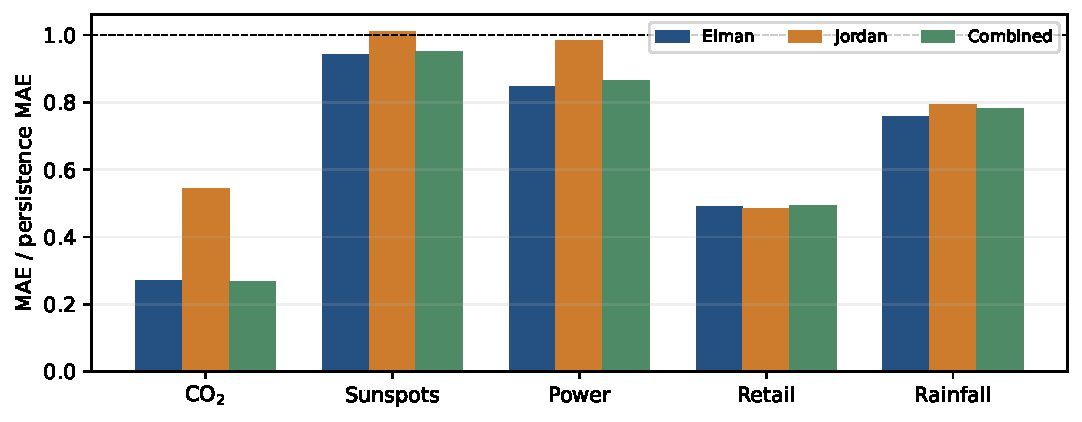
\includegraphics[width=0.82\textwidth]{skill.pdf}
\caption{Final-test network MAE relative to persistence MAE. The horizontal line denotes equal error. Lower ratios are better.}
\label{fig:skill}
\end{figure*}

The best neural forecast improved on persistence by 73.21\% for carbon dioxide, 5.67\% for sunspots, 15.26\% for power, 51.67\% for retail, and 24.17\% for rainfall. Retail's applicable seasonal-naive method was stronger than persistence, at 3.978 rather than 7.069 index points MAE. Against that stronger baseline, Jordan's retail improvement was 14.12\%. Seasonal-naive was weaker than persistence for carbon dioxide, power, and rainfall. Jordan sunspots had 14.366 MAE, which exceeded persistence's 14.219; the required architecture did not always add practical skill. The absence of a fixed seasonal-naive solar benchmark follows from its variable cycle rather than from a zero baseline error. These ratios depend on the chosen diagnostic rules and do not measure economic or operational value.

MASE supplies a second scale-independent check. The best network's final MASE was 0.302 for carbon dioxide, 0.667 for sunspots, 0.586 for power, 0.654 for retail, and 0.801 for rainfall. Each value was below one relative to the training-period first-difference scale. A MASE below one here means that the model's test MAE was below that fixed training reference; it does not mean that it beat every test-period naive method. In particular, retail's seasonal baseline and sunspots' persistence should be read directly from Table~\ref{tab:baselines}. The five denominators were estimated from different histories and are not interchangeable measures of task difficulty.

\subsection{Representative Forecast Behaviour and Limits}
Figure~\ref{fig:examples} shows the final 70 scored target positions for carbon dioxide and retail using the lowest-mean-MAE architecture in each case. Each blue line averages the three seed forecasts for display only; Tables~\ref{tab:performance} and \ref{tab:baselines} use the saved seed-level forecasts. This post-hoc display illustrates where a small average error may coexist with larger individual misses and did not affect selection.

\begin{figure*}[t]
\centering
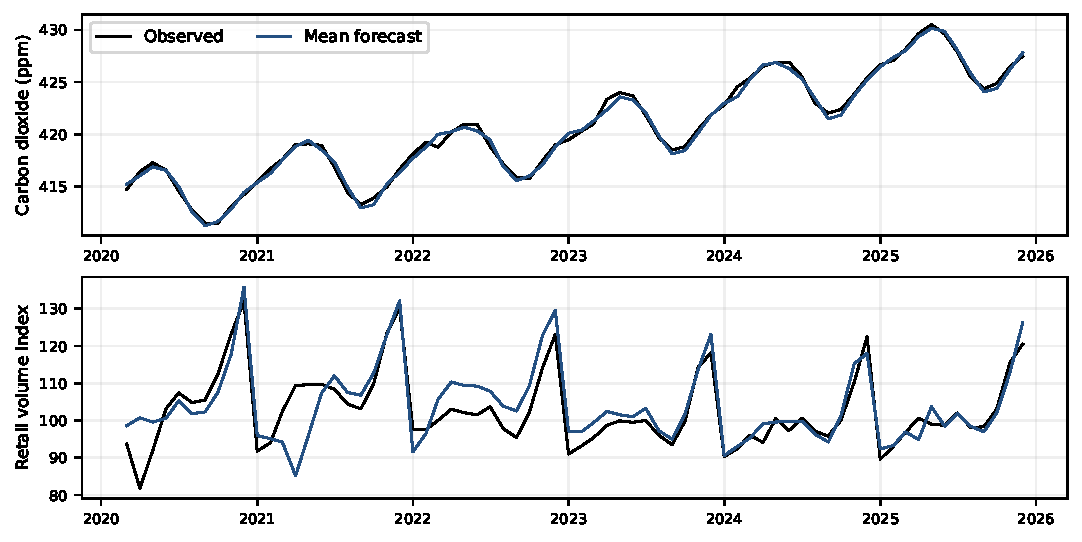
\includegraphics[width=0.86\textwidth]{examples.pdf}
\caption{Observed levels and mean forecasts for the final 70 scored carbon-dioxide and retail targets. The selected combined network is shown for carbon dioxide and Jordan for retail.}
\label{fig:examples}
\end{figure*}

The carbon-dioxide panel tracks the rising observed level while retaining some monthly error. The retail panel shows larger misses around sharp changes, consistent with its RMSE of 5.121 exceeding its MAE of 3.416. The largest retail absolute error in one displayed seed was 24.28 index points in April 2021. This outlier illustrates how a changing level can dominate squared-error measures, but a single miss does not establish the general cause of error. The panels omit earlier test origins and show a seed-mean trajectory; they should not be treated as independent or additional evaluations.

The cross-series evidence supports a narrower conclusion than a universal winning architecture. Elman had the lowest observed MAE on three series, combined feedback on one, and Jordan on one. The combined path never produced a large final advantage over Elman under the frozen grid, even though it added trainable weights. Conversely, the larger Elman--Jordan differences on carbon dioxide and power showed that nominally similar parameter counts did not guarantee similar predictions. The finite architecture-specific search, three seeds, fixed input histories, and one final period per series limit the generality of both statements. Repeated origins within a series were temporally dependent, so the study did not treat their errors as independent samples for a significance test.
